\subsection{Zipf's Law Application}
\index{Zipf's Law}
\index{Zipf's Law!Application}
\index{Applications!Zipf's Law}

$Revision: 1.15 $

Originally written on February 7, 2003.

\paragraph{The Program}

%is Java has built-in \api{StreamTokenizer}; you just have
%to instruct it how you want tokens to look like, and get
%them from any input stream, one-by-one. Java also provides
%us with built-in types and data-structures to manage
%collections (build, sort, store/retrieve) efficiently.

\paragraph{Data Structures}

The main statistics ``place-holder'' is a \api{oStats} \api{Hashtable}, nicely
provided by {\java}, which hashes by words as keys to other
data structures, called \api{WordStats}. The \api{WordStats} data structure
contains word's spelling, called lexeme (borrowed this term
from compiler design), word's frequency (initially $0$), and
word's rank (initially $-1$, i.e. unset). \api{WordStats} provides a typical
variety of methods to access and alter any of those three values.
There is an array, called \api{oSortedStatRefs}, which will eventually
hold references to \api{WordStats} objects in the \api{oStats} hashtable in
the sorted by the frequency.

Hashtable entry might look like this in pseudo-notation:

\verb+{ <word> } -> [ WordStats{ <word>, <f>, <r> } ]+

\subsubsection{Mini User Manual}

\paragraph{System Requirements}

The program was mostly developed under Linux, so there's
a \file{Makefile} and a testing shell script to simplify some routine tasks.
For JVM, any JDK 1.4.* and above will do. \tool{bash} would be nice
to have to be able to run the batch script. Since the application
itself is written in {\java}, it's not bound to specific architecture,
thus may be compiled and run without the makefiles and scripts
on virtually any operating system.

\paragraph{How To Run It}

There are at least three ways how to run the program, listed in order of complexity
(in terms of number of learning and typing involved).
In order for the below to work you'd need some corpora in
the same directory as the application.

\paragraph{Using the \tool{testing.sh} Script}

The script is written using \tool{bash} syntax; hence, \tool{bash} should be
present. The script ensures
that the program was compiled first, by invoking \tool{make}, then
in a for loop feeds all the \file{*.txt} files (presumably our corpora) along with the \file{ZipfLaw.java}
program itself to the executable, one by one, and redirects its standard output
to the files as \file{$<$corpus-name$>$[$<$options>$]$.log} in the current directory. These files will contain the
grouping of the 100 most frequent words every 1000 words as well as frequency-of-frequency counts at the end.

\noindent
Type:

\verb+./testing.sh+

\noindent
to run the batch through with the default settings.

\verb+./testing.sh <options>+

\noindent
to override the default settings with $<$options$>$. $<$options$>$ are the same
as that of the \api{ZipfLaw} application (see \ref{sect:zipf-law-app}).

\paragraph{Using \file{Makefile}}

If you want to build and to run the application just for individual,
pre-set corpora, use the \tool{make} utility provided with UNIXen.

Type (assuming GNU-style \tool{make}, or \tool{gmake}):

\noindent
\verb+make+

	to just compile the thing

\noindent
\verb+make <corpus-name> [ > <filename>.log ]+

	to (possibly compile if not done yet) and run it for the corpus
	\verb+<corpus-name>+ and to optionally redirect output to the file
	named \verb+<filename>.log+
	The \verb+<corpus-name>+ are described in the \file{Makefile} itself.

\noindent
\verb+make clean+

	to clean up the \file{*.class} and \file{*.log} files that happened to be
	generated and so on.

\noindent
\verb+make run+

	is actually equivalent to running \tool{testing.sh} with no options.

\noindent
\verb+make report+

	to produce a PDF file out of the {\LaTeX} source of the report.

\paragraph{Running The ZipfLaw Application}
\label{sect:zipf-law-app}

You can run the application itself without any wrapping scripts
and provide options to it. This is a command-line application,
so there is no GUI associated with it yet. To run the application
you have to compile it first. You can use either \tool{make} with no
arguments to compile or use the standard Java compiler.

\noindent
\verb+make+

or

\noindent
\verb+javac -cp marf.jar:. ZipfLaw.java+

\noindent
After having compiled the thing, you can run it with the JVM.
There is one required argument - either corpus file to analyze
or \verb+--help+. If it's a corpus, it
may be accompanied with one or more options overriding the default
settings. Here are the options as per the application's output:

\vspace{15pt}
\hrule
\begin{verbatim}
Usage:
    java ZipfLaw --help | -h | [ OPTIONS ] <corpus-file>
    java ZipfLaw --list [ OPTIONS ] <corpus-file>

Options (one or more of the following):
    --case  - make it case-sensitive
    --num   - parse numerical values
    --quote - consider quotes and count quoted strings as one token
    --eos   - make typical ends of sentences (<?>, <!>, <.>) significant
    --nolog - dump Zipf's law graph values as-is instead of log/log
    --list  - lists already pre-collected statistics for a given corpus

\end{verbatim}

\hrule
\vspace{15pt}

If the filename isn't specified, that will be stated and the usage
instructions above displayed.
The output filename generated from the input file name with the
options (if any) pre-pended and it ends with the extension of \file{.csv},
which can directly be opened by OpenOffice Calc or Microsoft Excel.

\subsubsection{Experiments}

Various experiments on diverse corpora were conducted to find
out whether Zipf's Law can possibly fail. For that purpose
I used the following corpora:

\begin{itemize}
\item a technical white paper of Dr. Probst (\cite{probst95}) of 20k in size, the filename is \file{multiprocessor.txt}
\item three ordinary corpora (non-technical literature)
	(\cite{greif, ulysses, speak}) -- \file{grfst10.txt}, 853k;
	\file{ulysses.txt}, 1.5M; and \file{hwswc10.txt}, 271k
\item my personal mailbox in UNIX format, raw as is, 5.5M
\item the source code of this application itself, \file{ZipfLaw.java}, 8.0k
\end{itemize}


\paragraph{Default Setup}

This is very simplistic approach in the application, where
everything but a letter (26 caps, and 26 lowercase) is a
blank, and as such is discarded. All the words were folded to the
lower case as well. This default setup can be overridden by
specifying the command-line options described above.

\paragraph{Extreme Setup}

One of the option combinations, that makes the program
case-sensitive, considers the numbers, and treats ``!'',
``.'', and ``?'' as special tokens.

\subsubsection{Results}

We failed to prove Zipf wrong. With {\bf any} of the corpora and the settings.
Further, the log/log graphs of the frequency and the rank
for the default and the extreme setup are provided. The graphs don't change very much
in shape. For other option combinations, the graphs are not provided
since they don't vary much.
It turned out to be the that capitalization, end of sentence symbols,
and numbers, if treated as tokens, don't make much of a difference,
as if they simply aren't there.

In the distribution archive, you will find the \file{*.log} and \file{*.csv} files
of the test runs, which contain the described statistics. You are welcome
to do \verb+make clean+ and re-run the tests on your own. NOTE, by default
the output goes to the standard output, so it's a good idea to redirect
it to a file especially if a corpus is a very large one.

\paragraph{Graphs, The Default Setup}

\begin{figure}[h!]
	\begin{center}
	\includegraphics[width=0.5\textwidth]{grfst10_txt_default.png}
	\caption{Zipf's Law for the ``Greifenstein'' corpus with the default setup.}
	\end{center}
\end{figure}

\begin{figure}
    \begin{center}
    \includegraphics[width=0.5\textwidth]{hwswc10_txt_default.png}
    \caption{Zipf's Law for the ``How to Speak and Write Correctly'' corpus with the default setup.}
    \end{center}
\end{figure}

\begin{figure}
    \begin{center}
    \includegraphics[width=0.5\textwidth]{mokhov_default.png}
    \caption{Zipf's Law for my 5.6 Mb INBOX with the default setup.}
    \end{center}
\end{figure}

\begin{figure}
    \begin{center}
    \includegraphics[width=0.5\textwidth]{multiprocessor_txt_default.png}
    \caption{Zipf's Law for the white paper ``The United States Needs a Scalable Shared-Memory Multiprocessor, But Might Not Get One!'' with the default setup.}
    \end{center}
\end{figure}

\begin{figure}
    \begin{center}
    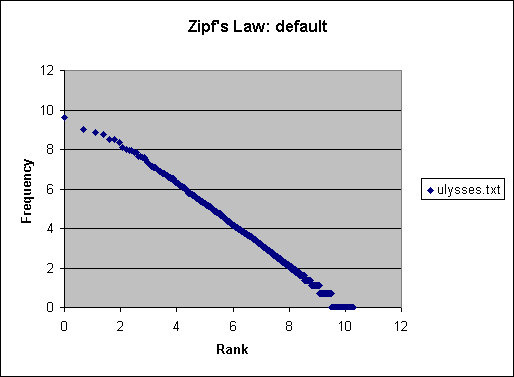
\includegraphics[width=0.5\textwidth]{ulysses_txt_default.png}
    \caption{Zipf's Law for the ``Ulysses'' corpus with the default setup.}
    \end{center}
\end{figure}

\begin{figure}
    \begin{center}
    \includegraphics[width=0.5\textwidth]{ZipfLaw_java_default.png}
    \caption{Zipf's Law for the ``ZipfLaw.java'' program itself with the default setup.}
    \end{center}
\end{figure}


\clearpage

\paragraph{Graphs, The Extreme Setup}

\begin{figure}[h!]
    \begin{center}
    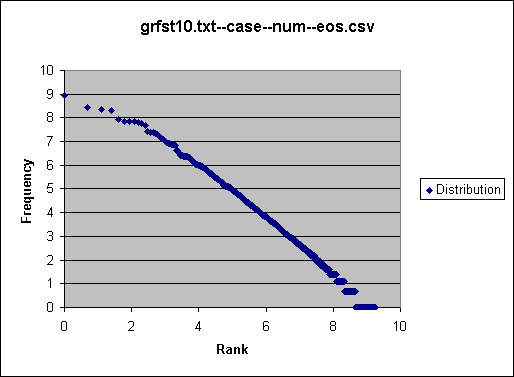
\includegraphics[width=0.5\textwidth]{grfst10_txt_case_num_eos.png}
    \caption{Zipf's Law for the ``Greifenstein'' corpus with the extreme setup.}
    \end{center}
\end{figure}

\begin{figure}
    \begin{center}
    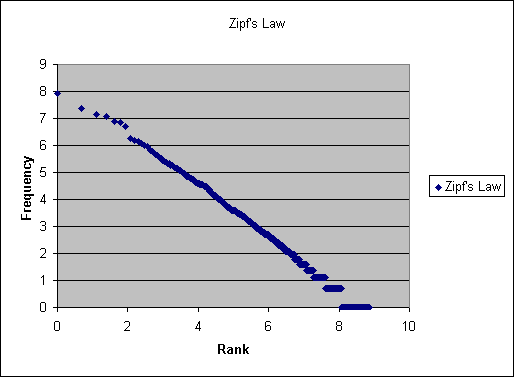
\includegraphics[width=0.5\textwidth]{hwswc10_txt_case_num_eos.png}
    \caption{Zipf's Law for the ``How to Speak and Write Correctly'' corpus with the extreme setup.}
    \end{center}
\end{figure}

\begin{figure}
    \begin{center}
    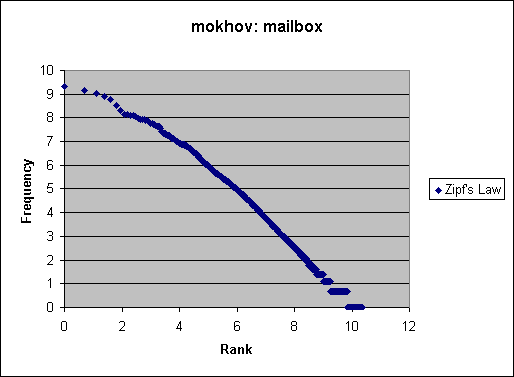
\includegraphics[width=0.5\textwidth]{mokhov_case_num_eos.png}
    \caption{Zipf's Law for my 5.6 Mb INBOX  with the extreme setup.}
    \end{center}
\end{figure}

\begin{figure}
	\begin{center}
	\includegraphics[width=0.5\textwidth]{multiprocessor_txt_case_num_eos.png}
	\caption{Zipf's Law for the white paper ``The United States Needs a Scalable Shared-Memory Multiprocessor, But Might Not Get One! with the extreme setup}
	\end{center}
\end{figure}

\begin{figure}
	\begin{center}
	\includegraphics[width=0.5\textwidth]{ulysses_txt_case_num_eos.png}
	\caption{Zipf's Law for the ``Ulysses'' corpus with the extreme setup.}
	\end{center}
\end{figure}

\begin{figure}
	\begin{center}
	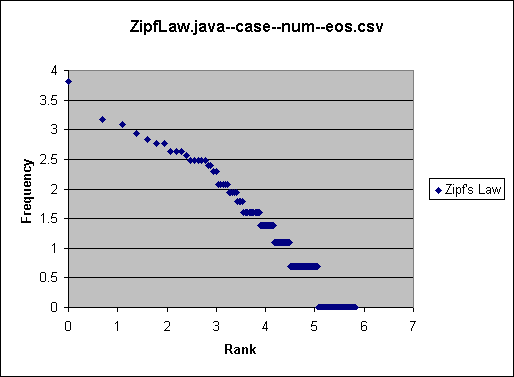
\includegraphics[width=0.5\textwidth]{ZipfLaw_java_case_num_eos.png}
	\caption{Zipf's Law for the ``ZipfLaw.java'' program itself with the extreme setup.}
	\end{center}
\end{figure}

\subsubsection{Conclusions}

Zipf's Law holds so far. However, more experimentation is required,
for example, other punctuation characters than
that ending a sentence were not considered. Then other languages than English is a good
area to explore as well.

% EOF
